\section{K-means}
\label{sec:kmeans}
This problem is called k-means because it aims to describe the \quoted{clustering} by separating the data into clusters ($\gls{sym:cluster}$), and define each cluster with it's mean ($\gls{sym:cent}$). Note that the mean of the cluster, from a phisical point of view, is the center of mass of the cluster itself as if it is composed my unitary point masses located at the datapoints positions. The mean is not necessarily a point belonging to the cluster.

Let's assume to have extrapolated $F$ features from each of our signals, to produce a set $\gls{sym:snapset}$ of $n$ {\gls{glo:snap}}s $\gls{sym:snap}_i, i \in [1,n], \gls{sym:snap}_i \in \gls{sym:snapset} $ (every {\gls{glo:snap}} is a vector of features $\in \mathbb{R}^F$). The task is to define a set $\gls{sym:cluster}$ of $k$ clusters ($k \leq n$) $\gls{sym:cluster}_i, i \in [1,k], \gls{sym:cluster}_i \in \gls{sym:cluster}$ that minimize the squared sum of the distances between the {\gls{glo:snap}}s and the centroids $\gls{sym:cent}_i$ of the clusters they belong to. This is equivalent to finding the centroids that minimize the \textbf{variance} of the clusters themselves, so the problem can be formulated as in the \autoref{eq:kmeans_problem}.

\begin{equation}
  \argmin{\gls{sym:cluster}}\sum_{i=1}^{k}\sum_{\gls{sym:snap}_j \in \gls{sym:cluster}_i} \norm{\gls{sym:snap}_j - \gls{sym:cent}_i}^2 = \argmin{\gls{sym:cluster}}\sum_{i=1}^{k}\abs{\gls{sym:cluster}_i}\mathrm{Var}\gls{sym:cluster}_i
  \label{eq:kmeans_problem}
\end{equation}

Unfortunately, this problem is NP-hard, even for as little as $F=2$ features considered \cite{MAHAJAN201213}, so it is not possible to guarantee to find the global optimum in a reasonable time.

Anyway, {\gls{glo:heuristic}} clustering algorithms were already developed in the 1950s. 
The first appearance of the term \quoted{K-means} was used in 1957 by MacQueen \cite{macqueen1967some}, and the algorithm settled to a \quoted{standard} version  published by Stuart Lloyd in 1982 \cite{Lloyd1982} (but developed at Bell Labs in 1957).

Among all the unsupervised clustering algorithms, a survey from 2002 \cite{berkhin2002survey} stated that K-means \quoted{is by far the most popular clustering algorithm used inscientific and industrial applications}. A more recent survey from 2019 \cite{Abla2019survey}, cithe this algorithm as first in the group of four most polular algorithms.

Nowadays, the K-means algorithm is implemented in many libraries, such as \texttt{scikit-learn} for \texttt{Python}, and others for \texttt{C}, \texttt{R}, \texttt{MATLAB}, etc. However, the runtime performances vary widely depending on the implementation \cite{Kmeans-performances-Kriegel2017}. The problem of the algorithm returning a local minima instead of the global one is still present. Most implementations try to minimize the probability of returning this sub-optimal result by running the algorithm multiple times with different initializations and then selecting the best result, so the problem of getting a sub-optimal resulti is not a common issue in practice.

\subsection{Training}

\begin{figure}[htbp]
  \centering
  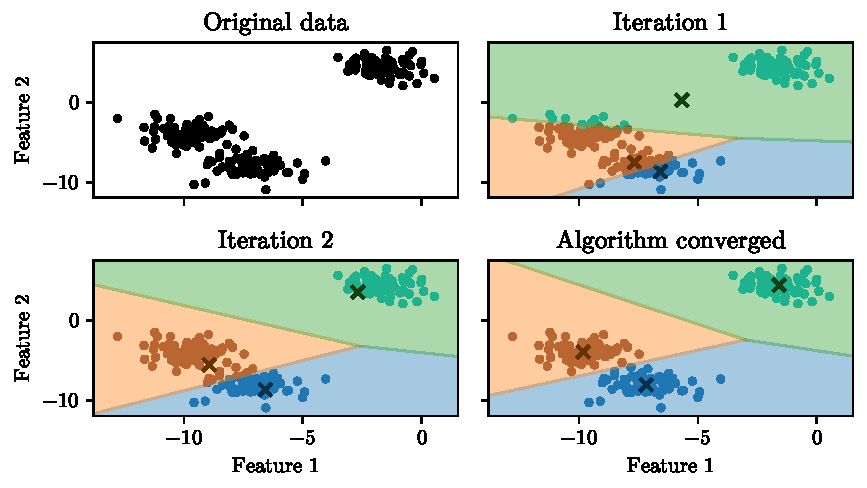
\includegraphics[width=\textwidth]{images/Kmeans_vornoi.pdf}
  \caption{K-means algorithm in the $2$-dimensional space}
  \label{fig:kmeans_vornoi}
\end{figure}

 The naive k-means algorithm consists of a series of iterations. First, the centroids $\gls{sym:cent}_i$ are initialized randomly, then the {\gls{glo:snap}}s are assigned to the nearest centroid, and finally, the centroids are updated as the mean of the {\gls{glo:snap}}s assigned to them. These steps are repeated until the position of the centroids does not change anymore, or a defined maximum number of iterations is reached. This naive algorithm is summarized in the \autoref{alg:kmeans}.

\begin{algorithm}
  \caption{Training of the K-means model}
  \label{alg:kmeans}
  \begin{algorithmic}[1]
    \Function{K-means.train}{$\gls{sym:snapset}, k$}
    \LineComment{$\gls{sym:snapset}$ is the set of snapshots to be clustered}
    \LineComment{$k$ is the number of clusters to be obtained}
    \State $\gls{sym:cent}_i \gets \text{random initialization}, \forall i \in [1,k], \gls{sym:cent}_i \in \text{Domain of }\gls{sym:snapset}$
    \Repeat
    \LineComment{Every snapshot is assigned to the nearest centroid. Every centroid defines a cluster containing the assigned snapshots}
    \State $\gls{sym:cluster}_i \gets \left\{ \gls{sym:snap}_p : \norm{\gls{sym:snap}_p - \gls{sym:cent}_i}^2 \leq  \norm{\gls{sym:snap}_p - \gls{sym:cent}_j}^2  \forall j \in [1,k] \right\} \forall i \in [1,k] $
    \LineComment{The centroids are updated as the mean of their snapshots}
    \State $\gls{sym:cent}_i \gets \frac{1}{\abs{\gls{sym:cluster}_i}}\sum_{\gls{sym:snap}_j \in \gls{sym:cluster}_i} \gls{sym:snap}_j, \forall i \in [1,k]$, \Comment{$\abs{\gls{sym:cluster}_i}$ is the cluster size}
    \Until{All the centroids do not change anymore, or max iterations reached}
    \State $r_i \gets \max{\norm{\gls{sym:snap}_j-\gls{sym:cent}_i}, \, \forall \gls{sym:snap}_j \in \gls{sym:cluster}_i}, \, \forall i \in [1,k]$
    \State \Return $\mathcal{M}_{\text{\texttt{k-means}}}$  \Comment{The model contains the centroids $\gls{sym:cent}_i$, the radii ${r}_i$ of the clusters, and the labels of the snapshots}
    \EndFunction
  \end{algorithmic}
\end{algorithm}

As an example, we can consider $F=2$ features, and generate some test points shaped like three separated clusters. In the \autoref{fig:kmeans_vornoi} are shown the original data, the first two iterations of the algorithm, and the final result. The K-means algorithm had $n=200$ snapshots, and $k=3$ clusters as input. The colors of the dots and the shaded areas represent the clusters and the decision boundaries. The centroids are represented as black crosses.
The decision boundaries are a Voronoi tessellation of the space, and they are defined as the set of points that are equidistant from the centroids of two different clusters. The algorithm itself does not compute the boundaries, but it is useful to plot them for visualization purposes.

\subsection{Improvements to the K-means algorithm}
\label{sec:kmeans_improvements}
\paragraph*{Kmeans}
Finding the optimal solution of the k-means problem (\autoref{eq:kmeans_problem}), as said, is NP-hard.
To address this problem, some other {\gls{glo:heuristic}}s algorithms have been proposed in the last two decades. Simple implementations have time complexity $\mathcal{O}(n^2)$ \cite{Kmeans_linear}.  This means that the most algorithms do not scale well as the number $n$ of snapshot increases. With respect to the number of clusters, the problem has a linear complexity $\mathcal{O}(k)$.

It is worth noticing that an exact solution of the problem has been published \cite{Kmeans_vornoi_japan} with a time complexity $\mathcal{O}(n^{k\cdot F})$. This is still impractical for actual applications, as it is exponential with respect to both the number of clusters and the number of features $F$.

\paragraph*{Lloyd's algorithm}
The classic Lloyd algorithm \cite{Lloyd1982} has a complexity $\mathcal{O}(n\cdot k\cdot F )$.

\paragraph*{Various improvements to the Lloyd's algorithm} Keeping the same basic idea, various modifications of the Lloyd algorithm have been proposed to improve the performances. For example, Kanugo \cite{kanungo2004local} proposed a local search algorithm that has a complexity $\mathcal{O}(n^3)$. Another result by Malay \cite{Kmeans_linear} has a linear complexity $\mathcal{O}(n)$. 

Another inprovement has been developed by Elkan \cite{kmeans-accelerated}, by keeping track of the bounds from the instances (snapshots) and the centroids. This algorithm become convenient when number $k$ of clusters is large ($\geq 20$), and up to a dimensionality of $F=1000$ features.

A variant of the Lloyd algorithm regarding both the speed of execution and the memory consumption has been proposed by Sculley \cite{Sculley2010}. This solution achieve a reduction of the execution time by orders of magnitude, and enables to perform the classification even for datasets that dont't fit in the memory of the machine. This is achieved by using a \emph{mini-batch} approach, where the centroids are updated after each batch of snapshots.

With regard to the problem of converging to a local minimum, the most common approach is to run the algorithm multiple times with different initializations and then select the best result, this is avoided by Reddy \cite{Vornoi_Kmeans}, by using the vornoi tassellation of the hyperspace using the datapoints to generate the initialization for the centroid positions, this algorithm perform better in the sense that is less likely to get trapped in a local minima.


\paragraph{K-means\texttt{++}} 
The last improved algorithm reported in this section has it's own paragraph because it is the one used in this thesis. It was developed and named Kmeans\texttt{++} by Arthur and Vassilvitskii in 2007 \cite{Kmeanspp}. The difference from the Lloyd algorithm is only in the first initialization of the centroids $\gls{sym:cent}_i \forall i \in [1,n]$. In this case, instead of a random initialization for all the centroids, the first centroid $\gls{sym:cent}_1$ is chosen randomly from the snapshots, and then the other centroids are chosen from the remaining snapshots with a probability that depends from the distance of the candidate snapshot to the closest already chosen centroid. This approach is summarized in the \autoref{alg:kmeanspp}.

For the development of the framework of this thesis, the K-means\texttt{++} algorithm has been implemented in \texttt{Python}, using the \texttt{scikit-learn} library. The library function has been modified, adding a method that returns the radii of the clusters, this information is crucial for our scope, as it will be needed for evaluating if a new snapshot is a novelty, normal or fault, as it will be explained in the \autoref{sec:clust_metric} and \autoref{sec:clust_threshold}.

\begin{algorithm}
  \caption{K-means\texttt{++} algorithm}
  \label{alg:kmeanspp}
\begin{algorithmic}[1]
  \Function{K-means\texttt{++}.train}{$\gls{sym:snapset}, k$}
  \LineComment{$\gls{sym:snapset} = \{\gls{sym:snap}_1,\gls{sym:snap}_2, \dots , \gls{sym:snap}_n\}$ is the set of snapshots to be clustered}
  \LineComment{$k$ is the number of clusters to be obtained}
  \State $\gls{sym:cent}_1 \gets \text{random initialization}, \gls{sym:cent}_1 \in \gls{sym:snapset}$
  \For{$i \gets 2$ to $k$}
  \LineComment{$D(\gls{sym:snap})$ is the distance of the snapshot $\gls{sym:snap}$ from the closest centroid already chosen}
  \State $c_i \gets \gls{sym:snap}' \in \gls{sym:snapset} \text{ with probability } \frac{D(\gls{sym:snap}')^2}{\Sigma_{\gls{sym:snap}\in\gls{sym:snapset}}D(\gls{sym:snap})^2}$
  \EndFor
  \State perform the Lloyd algorithm using the calculated $\gls{sym:cent}_i, \forall i \in [1,k]$ as initialization, get the model.
  \State \Return $\mathcal{M}_{\text{\texttt{k-means}}}$  \Comment{The model contains the centroids $\gls{sym:cent}_i$, the radii ${r}_i$ of the clusters, and the labels of the snapshots}
  \EndFunction
\end{algorithmic}
\end{algorithm}

\subsection{Selecting the number of clusters}
It is important to notice that, even being an \emph{unsupervised} learning algorithm, the K-means algorithm needs to know the number of clusters $k$ in advance. There are some methods to decide what is the best number of clusters, but they usually need to perform more iterations of the algorithm with different values of $k$, and then compare the results. This task is hardly automatable so, during the training phase, the user has to decide the number of clusters to be used.

To compare the results of the different iterations, it is possible to use some metrics on the data and the centroids. The most common metrics are the \emph{inertia} and the \emph{silhouette score}, described in the following paragraphs.

\paragraph*{Inertia}
The inertia metric measures the total (sum) distance of each point belonging to a cluster from the centroid of the cluster itself, as shown in the \autoref{eq:inertia}. This is called inertia because, in the physical sense, it is the sum of the moment of inertia of each cluster if all the snapshots were considered as point masses (with unitary mass). This analogy is useful to understand that the lower the inertia, the more compact the clusters are.

Let's span $k \in [1,9]$ and plot the inertia of the clusters for each value of $k$, on the previous dataset. The result is shown in the \autoref{fig:kmeans_inertia}. As expected, the inertia decreases as the number of clusters increases. This is not a desirable behavior, if the aim is selecting the number of clusters, the best guess is to select (by eye or with some automatism) the Pareto optimal point (\glsxtrshort{pof}) of the curve \cite{pareto}. 

\begin{equation}
  \label{eq:inertia}
  I = \sum_{i=1}^{k}\sum_{\gls{sym:snap}_j \in \gls{sym:cluster}_i} \norm{\gls{sym:snap}_j - \gls{sym:cent}_i}^2
\end{equation}

\begin{figure}
  \begin{subfigure}{\textwidth}
    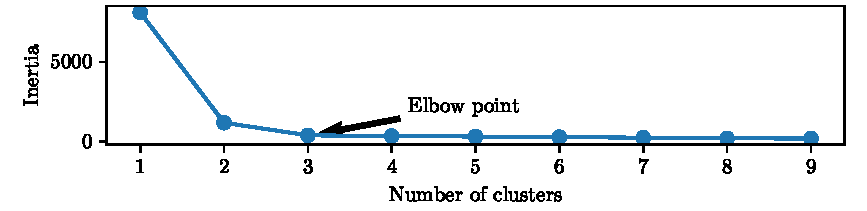
\includegraphics[width=\textwidth]{images/Kmeans_inertia.pdf}
    \caption{Inertia of the clusters for different values of $k$}
    \label{fig:kmeans_inertia}
  \end{subfigure}
  \begin{subfigure}{\textwidth}
    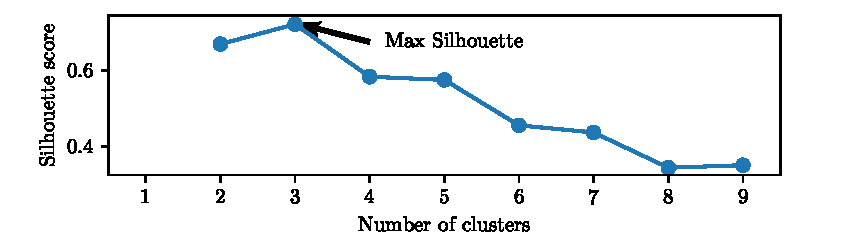
\includegraphics[width=\textwidth]{images/Kmeans_silhouette.pdf}
    \caption{Silhouette score of the clusters for different values of $k$}
    \label{fig:kmeans_silhouette}
  \end{subfigure}
  \label{fig:kmeans_metrics}
  \caption{Metrics for selecting the number of clusters}
\end{figure}

\paragraph*{Silhouette score}
A better metric that can be used to select the number of clusters is the silhouette score.
The silhouette score is defined for each snapshot as in \autoref{eq:silhouette}, where $a$ is the mean distance of the snapshot from the other snapshots in the same cluster, and $b$ is the mean distance of the snapshot from the snapshots in the nearest cluster. The resulting silhouette $S_i$ of a snapshot $\gls{sym:snap}_i$ is a scalar: $S_i \in [-1,1]$.
The three relevant cases are:
\begin{itemize}
  \item a value close to $1$ means that the snapshot is far inside its own cluster and far from snapshots of other clusters;
  \item a value close to $0$ means that the snapshot is on the boundary between two clusters;
  \item a value close to $-1$ means that the snapshot is far from its own cluster and close to another cluster, so it may have been misassigned.
\end{itemize}

\begin{equation}
  \label{eq:silhouette}
  S_i = \frac{b_i - a_i}{\max{(a_i,b_i)}}
\end{equation}

At this point, the global silhouette score $S_g$ can be computed as the mean of the silhouette scores of all the snapshots (\autoref{eq:silhouette_global}). The global silhouette score, for the same example dataset, is shown as a function of the number of clusters $k$ in the \autoref{fig:kmeans_silhouette}. Note that this time $k \in [2,9]$, because the silhouette score is not defined for a single cluster.

In this case, the best value for $k$ is $k=3$, because it is the value that maximizes the silhouette score. This approach is simpler and easier to automate than the inertia one. 

\begin{equation}
  \label{eq:silhouette_global}
  S_g = \frac{1}{n}\sum_{i=1}^{n} S_i
\end{equation}

\subsection{Assignation of the new instance to a cluster}
The procedure for assigning the new snapshot $\gls{sym:snap}_n$ to a cluster is quite simple, it is sufficient to compute the distance between $\gls{sym:snap}_n$ and the centroids $\gls{sym:cent}_m$, $\forall m \in  [1, \dots , k]$. The distance is defined as the $l^2$-norm in the feature space, it can be computed using the \autoref{eq:clust_dist}, and assign $\gls{sym:snap}_n$ to the cluster with the minimum distance.

\begin{equation}
  \label{eq:clust_dist}
  \gls{sym:dist}_{n,m} = ||\gls{sym:snap}_{n,f} - \gls{sym:cent}_{m,f}||_2 = \sqrt{\sum_{f=1}^{F} (\gls{sym:snap}_{n,f} - \gls{sym:cent}_{m,f})^2}
\end{equation}

\subsection{Evaluation of a new instance}

At this point, with a model trained on the data, a generic $n$th new snapshot instance $\gls{sym:snap}_n$ can be evaluated using the K-means algorithm.
From a geometric point of view, the snapshot $\gls{sym:snap}_n$ is a point in the ${F}$-dimensional space, where ${F}$ is the number of features used to train the model.

For demonstration purposes, in this section, since it is still feasible to show 3D plots, it is considered an example with ${F}=3$ features.

\begin{figure}[htbp]
  \centering
  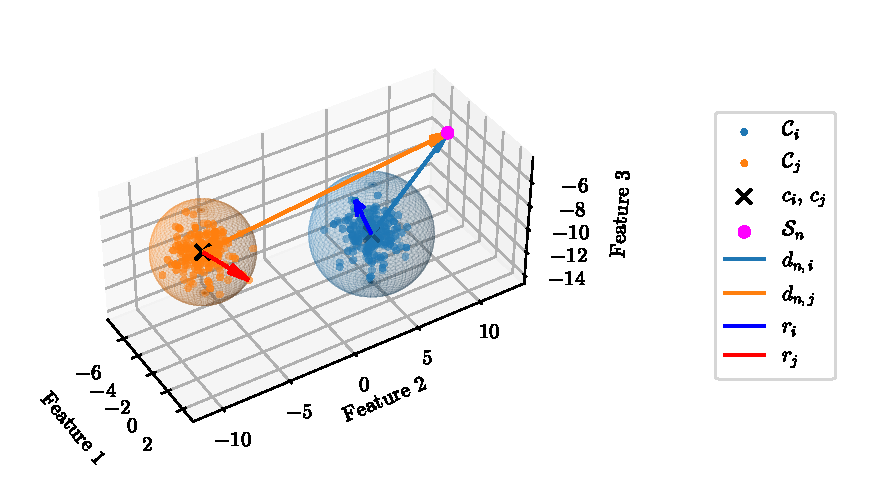
\includegraphics[width=\textwidth]{images/Spheres_2.pdf}
  \caption{Cluster model in the $3$-dimensional space, with new snapshot $\gls{sym:snap}_n$}
  \label{fig:clust_spheres}
\end{figure}

In the \autoref{fig:clust_spheres}, the training data are represented in the $3$-dimensional space, where the axis are the features used to train the model. The K-means model has been ideally trained with an arbitrary number $k$ of clusters but, for display purposes, only two clusters  ($\gls{sym:cluster}_i$ and $\gls{sym:cluster}_j$) are plotted.
\paragraph*{}
The entities shown in the \autoref{fig:clust_spheres} are:
\begin{itemize}
  \item $\gls{sym:cent}_{i(j)}$ is the centroid of the $i$th ($j$th) cluster;
  \item $\gls{sym:radius}_{i(j)}$ is the radius of the $i$th ($j$th) cluster, it is defined as the distance between the centroid $\gls{sym:cent}_{i(j)}$ and the farthest point belonging to the cluster itself;
  \item $\gls{sym:cluster}_{i(j)}$ is the set of training snapshots belonging to the $i$th ($j$th) cluster, it has a centroid $\gls{sym:cent}_{i(j)}$ and a radius $\gls{sym:radius}_{i(j)}$;
  \item $\gls{sym:snap}_n$ is the new snapshot to be evaluated;
  \item $\gls{sym:dist}_{n,i}$ is the vector between $\gls{sym:snap}_n$ and $\gls{sym:cent}_i$;
  \item $\gls{sym:dist}_{n,j}$ is the vector between $\gls{sym:snap}_n$ and $\gls{sym:cent}_j$;
  \item the semi-transparent spheres represent the cluster sizes, the radius of the spheres is the radius of the cluster itself, and the center is the centroid of the cluster;
\end{itemize}



\subsection{Metric for the new instance evaluation}
\label{sec:clust_metric}
Once the new snapshot $\gls{sym:snap}_n$ has been assigned to the right cluster $\gls{sym:cluster}_i$ using \autoref{eq:clust_dist}, some kind of measure (\gls{aka} metric) linked to how novel this snapshot is needs to be computed. In this document, this measure, referred to the $n$-th cluster, will be called $e_n$, in order to remind some sort of error, even if it is not an error in the strict sense. One simple approach could be to compute the difference between the distance of $\gls{sym:snap}_n$ from the centroid $\gls{sym:cent}_i$ and the radius $\gls{sym:radius}_i$ of the cluster itself. With this approach, the measure defined in the \autoref{eq:clust_eval} is relative to the current snapshot, so it is possible to use that as a novelty measure.

\begin{equation}
  \label{eq:clust_eval}
  e_{n} = ||\gls{sym:dist}_{n,i}||_2 - ||\gls{sym:radius}_{i}||_2, \text{ where $i$ is the of the assigned cluster}
\end{equation}

Few consideration about the resoult of the \autoref{eq:clust_eval}:
\begin{itemize}
  \item if $e_{n} > 0$, the new snapshot $\gls{sym:snap}_n$ is outside the sphere of radius $\gls{sym:radius}_i$ centered in $\gls{sym:cent}_i$, so it is probably a novel snapshot;
  \item if $e_{n} < 0$, the new snapshot $\gls{sym:snap}_n$ is inside the sphere of radius $\gls{sym:radius}_i$, so it is probably a normal snapshot. In this case, it is worth noticing that this assumption is reasonable only if the shape of the point cloud resembles a sphere, otherwise, the radius $\gls{sym:radius}_i$ is not a good measure of the cluster size, and use it for novelty detection would not be reasonable. \textbf{This emphasizes the importance of the standardization procedure applied to the features before the training phase};
\end{itemize}



Using this metric it is possible to define as \emph{novelty} all the snapshots with $e_{n} > 0$ and as \emph{normal} all the snapshots with $e_{n} < 0$. This approach is not very robust because s snapshot that is even slightly outside the sphere of radius $\gls{sym:radius}_i$ will be considered as novelty, but since the sphere is tuned the training \emph{measured} data, that have an aleatory component, this approach will probably detect some novelty even in normal snapshots.

\subsection{Introducing a threshold for the metric evaluation}
\label{sec:clust_threshold}
In order to improve the robustness of the novelty detection algorithm, it is possible to define a threshold ${t}_i$ for each cluster $\gls{sym:cluster}_i$ and use it to detect if a snapshot is a novelty or not. Once the threshold ${t}_i$ is defined, the detection of the novelty can be triggered by the condition $e_{n} > {t}_i$.

\paragraph*{}
At this point, the problem is that the user would have to define a threshold for each cluster, and this is not a trivial task. This is because it is likely that the clusters have different sizes, and so one threshold for all the clusters would be more conservative for the smaller clusters and less conservative for the bigger ones. Moreover, most of the times, the clusters shape and sized will not have a phisical meaning, and the act of manually define a threshold for each cluster would be against our goal of designing a fully unsupervised framework.

\paragraph*{}
To address this problem, it is possible to change the definition of the metric itself, so that is not dependent on the cluster size. This can be done by normalizing the already defined metric $e_{n}$ with the radius $\gls{sym:radius}_i$ of the cluster itself, as shown in the \autoref{eq:clust_eval_norm}. In this way, $t_i$ can be defined as a percentage of the cluster size, so that the user can define a single threshold for all the clusters, and selecting the number to assign to $t_i$ has a more intuitive meaning. From now on if not otherwise specified, the metric $e_{n}$ will be this normalized version.
Obviously, the metric can be easily displayed as a percentage: $e_{n,\%} = e_n \cdot 100$.
This value can be evaluated in real-time and plotted in a graph so that the user can see the novelty metric behavior over time.

\begin{equation}
  \label{eq:clust_eval_norm}
  e_{n} = \frac{\norm{\vect d_{n,i}}-\norm{\vect r_{n,i}}}{\norm{\vect r_{n,i}}} = \frac{\norm{\gls{sym:dist}_{n,i}}}{\norm{\gls{sym:radius}_{i}}} - 1, \text{ where $i$ is the of the assigned cluster}
\end{equation}

\subsection{Trasformation of the metric for the fault detection}
\label{sec:clust_fault}
In the previous \autoref{sec:clust_threshold} it has been proposed a metric to detect how novel a snapshot is.

Let's assume now to have trained the model on a dataset of snapshots collected in a period in wich the system was having a known malfunction. In this case, the metric applied to any future snapshot will carry the information of \quoted{how faulty} the system is, or better \quoted{how similarly the system is behaving \gls{wrt} a known malfunction}.

\begin{figure}[htbp]
  \centering
  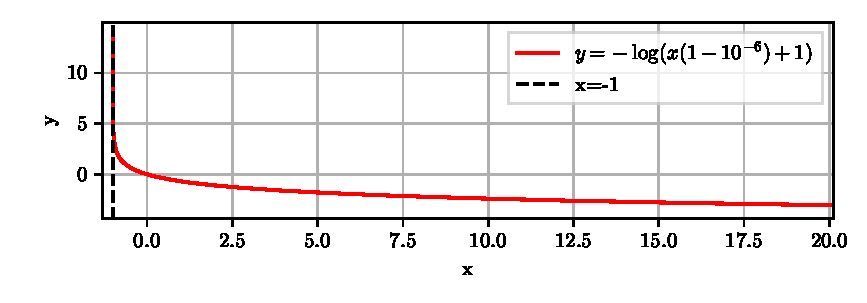
\includegraphics[width=\textwidth]{images/metric_trasform.pdf}
  \caption{Logarithmic Trasformation applied to the metric in case the model is working in fault detection mode}
  \label{fig:kmeans_fault}
\end{figure}


\subsection{Evaluation procedure}
The evaluation procedure developed to address the novelty/fault detection scope of this thesis can be summarized in the \autoref{alg:eval_new_snapshot}.

\begin{algorithm}
  \caption{Evaluation of a new snapshot with a K-means model}
  \label{alg:eval_new_snapshot}
  \begin{algorithmic}[1]
    \Procedure{eval}{$\mathcal{M}_{\text{\texttt{k-means}}},\gls{sym:snap}, t$}
    \LineComment{$\mathcal{M}_{\text{\texttt{k-means}}}$ is the trained K-means model}
    \LineComment{the model contain the centroids $\gls{sym:cent}_i$ and the radii $\gls{sym:radius}_i$ of the clusters}
    \LineComment{$\gls{sym:snap}$ is the new snapshot to be evaluated}
    \LineComment{$t$ is the threshold for the novelty detection}
    \State $k \gets \text{number of clusters in $\mathcal{M}_{\text{\texttt{k-means}}}$}$
    \State min $\gets \infty$ \Comment {initialize the minimum distance}
    \For{$i \gets 1$ to $k$}
    \State $\gls{sym:dist}_{i} \gets \gls{sym:snap} - \gls{sym:cent}_{i}$
    \If {$\norm{\gls{sym:dist}_{i}} < \text{min}$}
    \State min $\gets \norm{\gls{sym:dist}_{i}}$
    \State $i_{\text{min}} \gets i$
    \EndIf
    \EndFor
    \State$e \gets \frac{\norm{\gls{sym:dist}_{i_{\text{min}}}}}{\norm{\gls{sym:radius}_{i_{\text{min}}}}} - 1$ \Comment {compute the novelty metric}
    \If {$e > t$}
    \State \Return novelty  \Comment {the snapshot is novelty}
    \Else
    \State \Return normal \Comment {the snapshot is normal}
    \EndIf
    \EndProcedure
    %\end{small}
  \end{algorithmic}
\end{algorithm}


\subsection{Comment about selecting wrong value of $k$}
\label{sec:wrong_k}
A brief comment about what has been done in the experimental phase, in the cases where the number of clusters $k$ was difficult to define based on the silhouette plots. This happened when the maximum value of $k$ was shared between more than one value of $k$ (multiple peaks with similar values or a flat shape of the peak).

In this case, the best choice is to select the maximum value of $k$ that is still compliant with the silhouette criterion. This is because the in scope of this thesis the final goal is to detect novelty. 

For display purposes, let's consider an example in the plane ($F$ = 2), with a dataset that clearly have three distinct clusters. Looking at \autoref{fig:kmeans_wrongk} it is clear why it is better to select $k$ larger than the actual number of clusters, rather than selecting it too small. This is because, if $k$ is larger than the actual number of clusters, the algorithm will still be able to detect the novelty, but if $k$ is too small, somewhere the algorithm will be forced to join two clusters together, and the a new snapshot that happens to be in the middle of the two clusters will not be detected as novelty. 

In the case of the \autoref{fig:kmeans_wrongk}, the best actual number of clusters were $k=3$, so selecting $k=2$ the algorithm would have joined the two clusters on the right, and the new snapshot would not have been detected as novelty. On the other hand, selecting $k=4$, the algorithm would have correctly detected the novelty, even if onne cluster has been split in two.

\begin{figure}
  \centering
  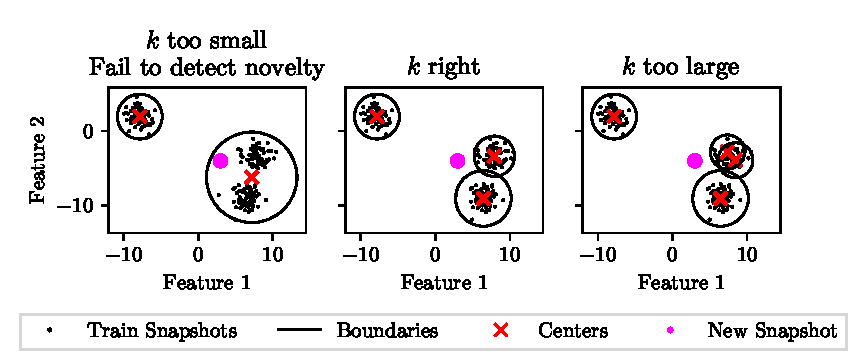
\includegraphics[width=\textwidth]{images/Kmeans_wrongk.pdf}
  \caption{Novelty detection of a new $\gls{sym:snap}_j$ with different values of $k$}
  \label{fig:kmeans_wrongk}
\end{figure}


\subsection{Limits of the kmeans algorithm}
This algorithm has many advantages: it's simple, popular (easy to find in libraries), it's fast, produces a model that does not need to store the original data in order to perform the classification of a new instance and it is well scalable. But it has also some limits, the most important are \cite[p273]{hands-on-geron2022}:
\begin{itemize}
  \item it perform poorely if the clusters are not spherical;
  \item it performs poorly if the clusters have very different sizes;
  \item it performs poorly if the clusters have different densities.
\end{itemize}

For this reason it is very important to perform a good preconditioning of the data. In this thesis, the data are \gls{glo:std} before the training phase, this makes the clusters more spherical and with similar sizes. 



